\documentclass[handout]{beamer}
\usepackage[T1]{fontenc}
\usepackage[utf8]{inputenc}
\usepackage{tikz-cd,wrapfig}
\usepackage{tcolorbox}
\usepackage{listings}

% Maths
\usepackage{amsmath}
\usepackage{amssymb}
\usepackage{physics}
\usepackage{siunitx}

% Backup slides
\newcommand{\backupbegin}{
    \newcounter{finalframe}
    \setcounter{finalframe}{\value{framenumber}}
}
\newcommand{\backupend}{
    \setcounter{framenumber}{\value{finalframe}}
}

% Infos
\title{Bubbles in a ferromagnetic superfluid}
\author{\\\textbf{Candidate:} Giorgio Micaglio\\ \textbf{Supervisor:} dr.\ Alessandro Zenesini }
%\subtitle{}
\date{March 10, 2025}
\institute{\\~\\Bachelor's Degree in Physics}
%\titlegraphic{...} 

%Bibliography
\usepackage[style=numeric, maxnames=4,backend=bibtex]{biblatex}
% other styles: numeric author title
\addbibresource{biblio.bib}
\DeclareBibliographyCategory{fullcited} %for not citing in bibliography
\newcommand{\mybibexclude}[1]{\addtocategory{fullcited}{#1}}

% Theme settings
\usetheme[physics]{beunitn}
\usecolortheme{rose}
\setbeamercovered{dynamic}


\begin{document}

\begin{frame}[plain]
    \maketitle
\end{frame}

\begin{frame}{Overview}
    \begin{columns}
        \begin{column}{0.6\textwidth}
            \begin{itemize}
                \item \textbf{Introduction}
                \item \textbf{Theoretical background}: Ferromagnetism in coherently coupled BEC spin-mixtures
                \item \textbf{Data analysis}: Characterization of false vacuum decay bubbles
                \item \textbf{Conclusions}
            \end{itemize}
        \end{column}
        \begin{column}{0.4\textwidth}
            \begin{figure}
                \centering
                \includegraphics[width=\linewidth]{../thesis/figures/chap1/artistic.png}
            \end{figure}
        \end{column}
    \end{columns}
\end{frame}

\begin{frame}{Introduction}
    Why \textbf{bubbles} in a ferromagnetic superfluid?

    First \textbf{experimental observation} of false vacuum decay (FVD) in the Pitaevskii BEC Center laboratories of the University of Trento.

    FVD provides information on \textbf{metastability} and is studied from quantum systems to cosmology

    Framework: \textbf{quantum spin mixture} optically trapped and cooled below the condensation temperature

    Bubbles originate in 
\end{frame}

% \section{Theoretical background}

\begin{frame}{Theoretical background: Ideal Bose gas}
    The ideal Bose gas is a quantum system of $N$ non-interacting bosons, described by statistical mechanics.
    \begin{equation*}
        \langle n_i \rangle = \frac{1}{e^{\beta(\epsilon_i - \mu)}-1}
    \end{equation*}
    \onslide<2->
    The occupation number of the ground state $N_0 = \langle n_0\rangle$ corresponds to the condensation. There is a phase transition at $T = T_c$.
    \begin{equation*}
        \frac{N_0}{N} = 1-\left(\frac{T}{T_c}\right)^\alpha \quad \text{for } T < T_c
    \end{equation*}
    In a finite box $\alpha = 3/2$, in harmonic confinement $\alpha = 3$.
\end{frame}

\begin{frame}{Theoretical background: Gross-Pitaevskii equation}
    A system of weakly-interacting bosons can be described by a single wavefunction by a mean-field approximation, yielding the GPE
    \begin{equation*}
        i\hbar \pdv{\psi(x,t)}{t} = \left[ 
            -\frac{\hbar^2}{2m}\nabla^2 + V(x,t) + g|\psi(x,t)|^2
        \right] \psi(x,t)
    \end{equation*}
    \onslide<2->
    In the stationary case
    \begin{equation*}
        \left[ 
            -\frac{\hbar^2}{2m}\nabla^2 + V(x) + g|\psi(x)|^2
        \right] \psi(x) = \mu \psi(x)
    \end{equation*}
    When the interaction dominates on the kinetic term
    \begin{equation*}
        n(x) = \frac{\mu - V(x)}{g}
    \end{equation*}
\end{frame}

\begin{frame}{Theoretical background: Two-component mixtures}
    The GPEs are coupled because of the inter-species interaction constant
    \begin{align*}
        &\left[ -\frac{\hbar^2}{2m}\nabla^2 + V(x) + g_{aa}|\psi_a(x)|^2 + g_{ab}|\psi_b(x)|^2
        \right] \psi_a(x) = \mu_a \psi_a(x) \\
        &\left[ -\frac{\hbar^2}{2m}\nabla^2 + V(x) + g_{ab}|\psi_a(x)|^2 + g_{bb}|\psi_b(x)|^2
        \right] \psi_b(x) = \mu_b \psi_b(x)
    \end{align*}
    Depending on the values of $g_{aa}$, $g_{bb}$ and $g_{ab}$, the system GS can behave in different manners
\end{frame}

\begin{frame}{Theoretical background: Two-component mixtures}
    The mixture can be miscible or immiscible: buoyancy effect
    \begin{figure}
        \centering
        \includegraphics[width=\textwidth]{../thesis/figures/chap1/buoyancy.png}
    \end{figure}
\end{frame}

\begin{frame}{Theoretical background: Coherent coupling}
    Coupling radiation between $\ket{a}$ and $\ket{b}$:
    \[
        \Omega_R(t)\exp{-i\omega_{\rm cpl}t+\phi} \quad \omega_{\rm cpl} = \omega_{ab} + \delta_B
    \]

    Double-well energy landscape
    \begin{equation*}
        E_{\rm MF}(Z) = -\hbar\left(|\delta g|n Z^2 + 2\Omega_R \sqrt{1-Z^2} + 2\delta_{\rm eff} Z\right)
        \label{eq:E_MF}
    \end{equation*}

    The order parameter is the ratio $|\delta g|n/\hbar\Omega_R$
\end{frame}

\begin{frame}{Theoretical background: Ferromagnetism}
    \begin{figure}
        \centering
        \includegraphics[width=\textwidth]{../thesis/figures/chap1/ferro.png}
    \end{figure}
\end{frame}

\begin{frame}{Theoretical background: False Vacuum Decay}
    \begin{figure}
        \centering
        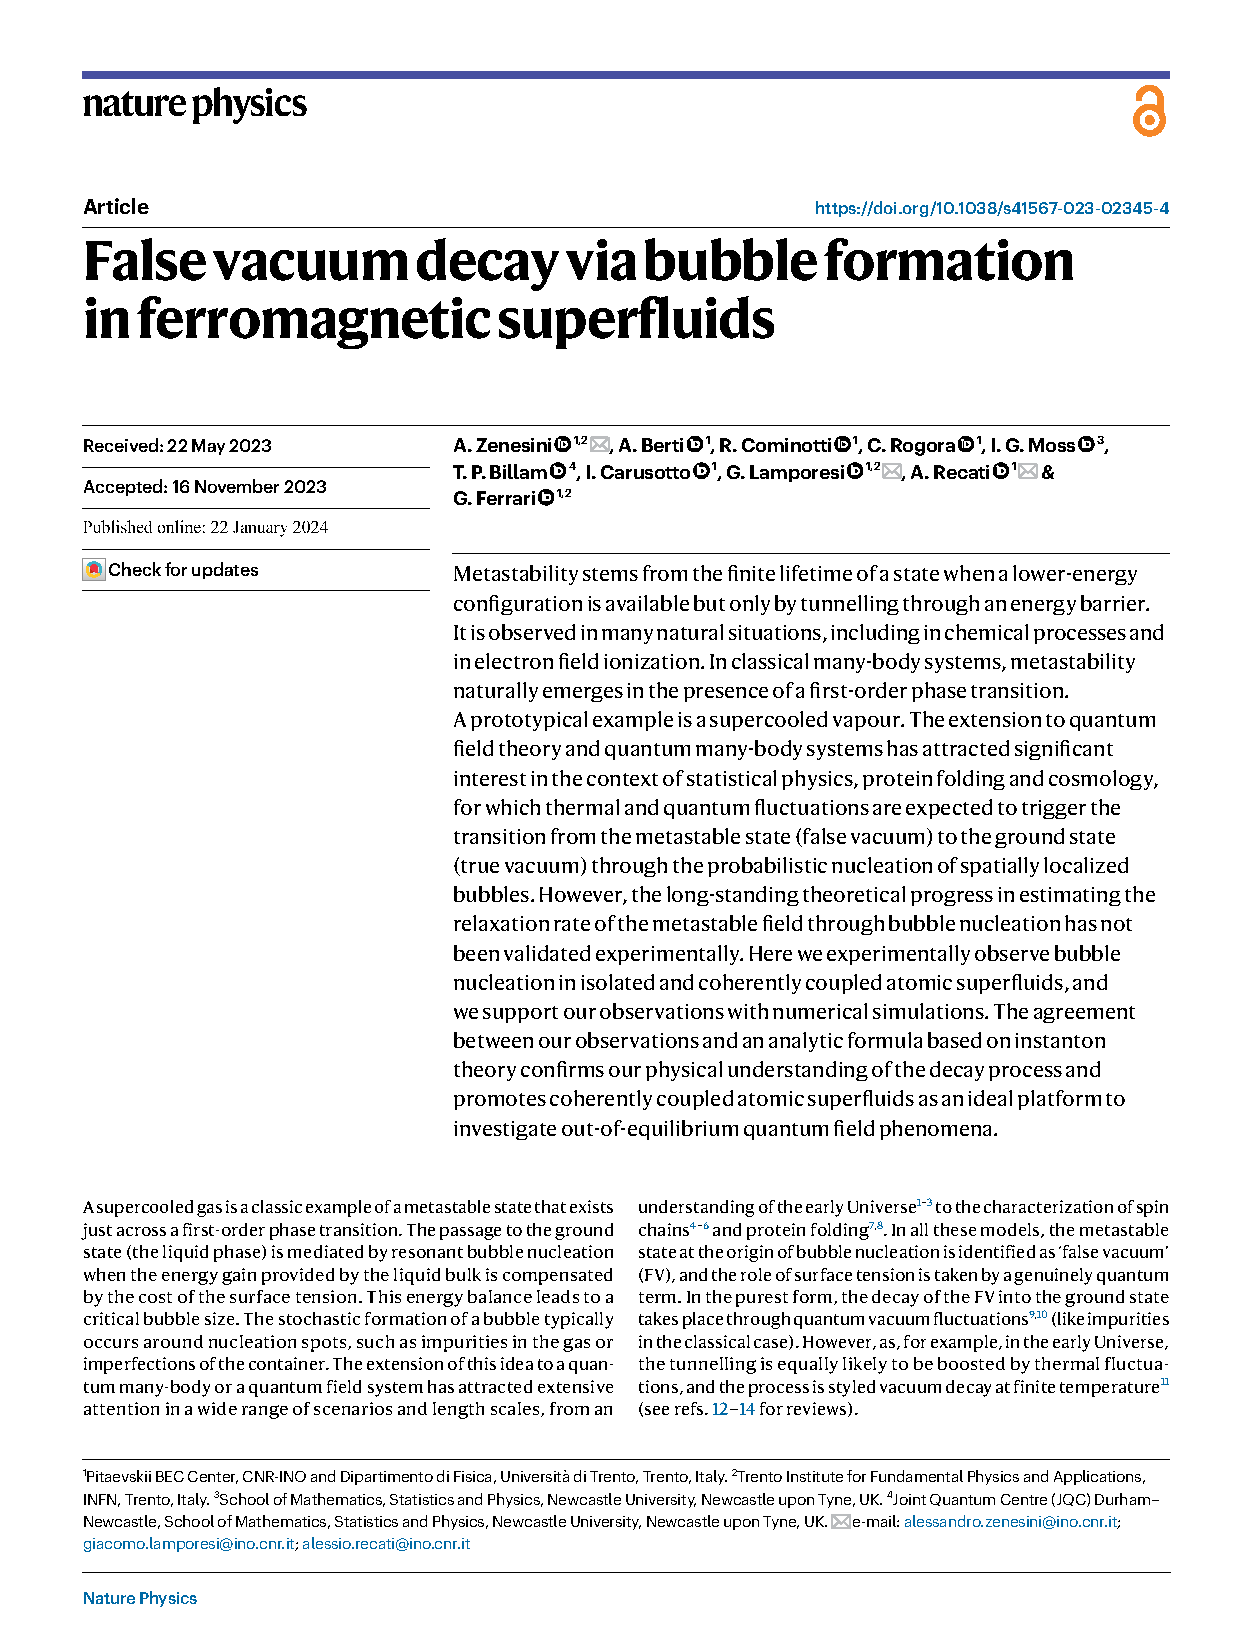
\includegraphics[width=0.8\textwidth]{../thesis/figures/chap1/FVD.png}
    \end{figure}    
\end{frame}

\begin{frame}{Data analysis: Experimental platform}
    The experiment uses $^{23}$Na atoms prepared in the state $\ket{F,m_F} = \ket{2, -2} = \ket{\uparrow}$, which is coupled to the state $\ket{1, -1} = \ket{\downarrow}$.

    The system is cigar-shaped with Thomas-Fermi radii 
    \begin{equation*}
        R_x = 200\ \unit{\micro\meter} \quad R_\rho = 2\ \unit{\micro\meter}
    \end{equation*}

    The magnetization is computed from the densities $n_\uparrow(x)$, $n_\downarrow(x)$
    \begin{equation*}
        Z(x) = \frac{n_\uparrow(x) - n_\downarrow(x)}{n_\uparrow(x) + n_\downarrow(x)}
    \end{equation*}
\end{frame}

\begin{frame}{Data analysis: Bubble fit}
    \begin{figure}
        \centering
        \includegraphics[width=\textwidth]{../thesis/figures/chap2/arctan_fit.png}
    \end{figure}
\end{frame}

\begin{frame}{Data analysis: Shot sorting}
    \begin{figure}
        \centering
        \includegraphics[width=\textwidth]{../thesis/figures/chap2/shot_sorting.png}
    \end{figure}
\end{frame}

\begin{frame}{Data analysis: Parameters clustering}
    \begin{figure}
        \centering
        \includegraphics[width=0.9\textwidth]{../thesis/figures/chap2/b_param_cluster.png}
    \end{figure}
\end{frame}

\begin{frame}{Data analysis: FFT and ACF}
    \begin{figure}
        \centering
        \includegraphics[width=0.9\textwidth]{../thesis/figures/chap2/inside_omdet.png}
    \end{figure}
\end{frame}

\begin{frame}{Data analysis: FFT and ACF}
    \begin{figure}
        \centering
        \includegraphics[width=\textwidth]{../thesis/figures/chap2/inside_fft_avg.png}
    \end{figure}
\end{frame}

\begin{frame}{Data analysis: ACF fits}
    \begin{figure}
        \centering
        \includegraphics[width=\textwidth]{../thesis/figures/chap2/fit_size_inside.png}
    \end{figure}
    \vspace{-0.5cm}
    \begin{figure}
        \centering
        \includegraphics[width=\textwidth]{../thesis/figures/chap2/fit_size_outside.png}
    \end{figure}
\end{frame}

\begin{frame}{Data analysis: ACF inside}
    \begin{figure}
        \centering
        \includegraphics[width=0.8\textwidth]{../thesis/figures/chap2/param_size_inside.png}
    \end{figure}
    \vspace{-0.5cm}
    \begin{figure}
        \centering
        \includegraphics[width=0.8\textwidth]{../thesis/figures/chap2/fit_omega_inside.png}
    \end{figure}
\end{frame}

\begin{frame}{Data analysis: ACF outside}
    \begin{figure}
        \centering
        \includegraphics[width=0.8\textwidth]{../thesis/figures/chap2/param_size_inside.png}
    \end{figure}
    \vspace{-0.5cm}
    \begin{figure}
        \centering
        \includegraphics[width=0.8\textwidth]{../thesis/figures/chap2/fit_omega_inside.png}
    \end{figure}
\end{frame}

\begin{frame}{Conclusions}
    
\end{frame}

\begin{frame}
    Thank you for your attention
\end{frame}

\backupbegin
\begin{frame}
    
\end{frame}
\backupend

\end{document}